% Bioinformatics Course Materials by David Weisman
% (Weisman@Computer.Org) is licensed under a Creative Commons
% Attribution-NonCommercial-ShareAlike 4.0 International License.

\RequirePackage[l2tabu, orthodox]{nag}

\documentclass[12pt]{tufte-handout}
\usepackage{amsmath}
\usepackage{array}
\usepackage{booktabs}
% \usepackage[top=1.0in,bottom=1.0in,left=1.0in,right=1.0in]{geometry}
\usepackage[pdftex]{graphicx}
\usepackage[utf8]{inputenc}
\usepackage{mathptmx}    % package times obsolete, see l2tabuen.pdf
% \usepackage[allowmove]{url}

\usepackage{tikz}
\usetikzlibrary{trees} 
\usepackage{microtype} % load /after/ mathptmx or other fonts

%To reduce widows and orphans, put in preamble:
    \raggedbottom                    %less likely orphans and widows
    \addtolength{\topskip}{0pt plus 10pt} % from FAQ
    \clubpenalty=10000
    \widowpenalty=10000


% Handy macros:
\newcommand{\set}[1]{\texttt{\{#1\}}}
\newcommand{\tnl}{\tabularnewline}
\newcommand{\ig}[2]{\includegraphics[#1]{#2}}  % insert graphics
\newcommand{\igw}[2]{\ig{width=#1\textwidth}{#2}}   % insert graphics width
\renewcommand{\theequation}{\textcolor{blue}{Equation \arabic{equation}}}

    \definecolor{shadecolor}{rgb}{1.0,1.0,0.8}


    \usepackage{soul}

    \definecolor{lightyellow}{rgb}{1,1,0.7}
    \sethlcolor{lightyellow}



% Question with counter
\newcounter{QuestionCounter}
\newcommand{\Question}[1]{\bigskip
\refstepcounter{QuestionCounter}

    {                           % local environment because left/rightskip change state
      \addtolength{\leftskip}{1cm}
      \addtolength{\rightskip}{1mm}
      \setlength{\parindent}{0mm}
      \setlength{\parskip}{1em}
      \textbf{Group Question \theQuestionCounter:} 
      #1
      \par
    }

\bigskip
}



% BEGIN probability tree

\makeatletter
% level 1
\define@key{pTree}{pl}{\def\pTree@pl{\color{blue}\ensuremath{#1}}}
\define@key{pTree}{pr}{\def\pTree@pr{\color{blue}\ensuremath{#1}}}
\define@key{pTree}{l}{\def\pTree@l{\color{blue}#1}}
\define@key{pTree}{r}{\def\pTree@r{\color{blue}#1}}

% level 2
\define@key{pTree}{pll}{\def\pTree@pll{\color{red}\ensuremath{#1}}}
\define@key{pTree}{plr}{\def\pTree@plr{\color{red}\ensuremath{#1}}}
\define@key{pTree}{prl}{\def\pTree@prl{\color{red}\ensuremath{#1}}}
\define@key{pTree}{prr}{\def\pTree@prr{\color{red}\ensuremath{#1}}}

\define@key{pTree}{ll}{\def\pTree@ll{\color{black}\textbf{#1}}}
\define@key{pTree}{lr}{\def\pTree@lr{\color{black}\textbf{#1}}}
\define@key{pTree}{rl}{\def\pTree@rl{\color{black}\textbf{#1}}}
\define@key{pTree}{rr}{\def\pTree@rr{\color{black}\textbf{#1}}}

\define@key{pTree}{pjll}{\def\pTree@pjll{\color{black}\ensuremath{\mathbf{#1}}}}
\define@key{pTree}{pjlr}{\def\pTree@pjlr{\color{black}\ensuremath{\mathbf{#1}}}}
\define@key{pTree}{pjrl}{\def\pTree@pjrl{\color{black}\ensuremath{\mathbf{#1}}}}
\define@key{pTree}{pjrr}{\def\pTree@pjrr{\color{black}\ensuremath{\mathbf{#1}}}}

% TBD: add 3 probs as params of levelTwo
% levelTwo{priorName}{condName}{priorProb}{condProb}{jointProb}
    \newcommand{\levelTwo}[5]{$P(\text{#2}) = P({\text{#1}})
       \times P(\text{#2}  \mid  \text{#1}) = #3 \times #4 = #5$}

% mandatory keys: 
% level 1
% pl,pr: p(l), p(r)
% l,r: labels left, right
% pll, plr, prl, prr: 2nd level conditional probabilities
% ll, lr, rl, rr: 2nd level labels
% pjll, pjlr, pjrl, pjrr: 2nd level joint probabilities

\newcommand{\probTree}[1]{
  \setkeys{pTree}{#1}

\begin{fullwidth}
    \begin{tikzpicture}[grow=right,
                        level distance=3.5cm,
                        every child node/.style={anchor=west,tree node}, 
                        tree node/.style={rectangle, rounded corners, draw},
                        level 1/.style={sibling distance=35mm},
                        level 2/.style={sibling distance=17mm}
                        ]

        \node[tree node] {Start here}
          child {node {\pTree@l}
            child {node {
                   \levelTwo{\pTree@l}{\pTree@ll}{\pTree@pl}{\pTree@pll}{\pTree@pjll}}
              edge from parent node[anchor=north] {\pTree@pll}}
            child {node {
                   \levelTwo{\pTree@l}{\pTree@lr}{\pTree@pl}{\pTree@plr}{\pTree@pjlr}}
              edge from parent node[anchor=south] {\pTree@plr}}
            edge from parent node[anchor=north] {\pTree@pl} }
          child {node {\pTree@r}
            child {node {
                   \levelTwo{\pTree@r}{\pTree@rl}{\pTree@pr}{\pTree@prl}{\pTree@pjrl}}
              edge from parent node[anchor=north] {\pTree@prl}}
            child {node {
                   \levelTwo{\pTree@r}{\pTree@rr}{\pTree@pr}{\pTree@prr}{\pTree@pjrr}}
              edge from parent node[anchor=south] {\pTree@prr}}
            edge from parent node[anchor=south] {\pTree@pr}
          };
    \end{tikzpicture}
\end{fullwidth}
}
\makeatother

% END probability tree

\setlength{\parskip}{.5cm}
\setlength{\parindent}{0cm}

\raggedright
\title{Probability Lab for Biol-360 Bioinformatics}
\date{}

\usepackage{hyperref}      % must be LAST usepackage of preamble!!
   \everymath{\displaystyle}

\begin{document}

\maketitle
\section{Introduction}
\label{sec:introduction}

Today we're focusing on several core concepts of probability, and applying these concepts to bioinformatics.   Most people know informally that the probability of flipping a coin and getting a head is $1/2=0.5$.  \marginnote{Many organisms don't have 1:1:1:1 proportions of A:T:G:C in their genomes.  For example, the  unicellular alga \textit{Chlamydomonas reinhardtii} has an unusually high GC content of $\approx 62\%$.  For our simple examples, we're assuming that the four nucleotides have equal proportions in a genome.} By the same idea, the probability of picking a random nucleotide on a chromosome and hitting a guanine is $1/4=0.25$.  

First we have to define a few terms.  These terms show up throughout probability, so it's good to learn them now.

\subsection{Sample Space, Outcomes, and Events}
\label{sec:sample-space-events}


First a quick review from basic math: a \textbf{set} is a collection of things.  Here's a set of four nucleotides: \set{A,C,G,T}.  Notice that we wrote the set with curly braces, which is the standard math notation.

\Question{Write out a set of 3 organelles found in eucaryotic cells.  Be sure to use the standard math notation.}

\bigskip

\textbf{Sample space} is the set of all possible outcomes of an experiment.  For example, if we ran an experiment that picked a single random nucleotide from a genome, we could get any of the 4 nucleotides, so the sample space is the set \set{A,C,G,T}.

\Question{Really, really dumb question:  \marginnote{Don't overthink this question!  It's really dumb, but you'll soon see where this is going.} How many entries are in the sample space \set{A,C,G,T}?}

\Question{\marginnote{A \textbf{dinucleotide} is a pair of nucleotides, for example, \texttt{TC}}What is the sample space of all possible dinucleotides? (Write it out.)  In other words, what are all the possible dinucleotides you might find in a big genome?}

\Question{How big is the sample space of dinucleotides?}

\Question{Now, Google to find a chart of the standard triplet genetic code, like we discussed in class last week.

What is the relationship between the standard genetic code, and the sample space of trinucleotides?}

\Question{How large is the sample space of trinucleotides?}

\Question{Using the ideas from above, derive a simple math function that takes a number of nucleotides and gives you the sample space size.   

Check your formula on the single, di-, and tri-nucleotide sample spaces in the earlier questions.  Now \marginnote{Biologist call this a \textbf{20-mer oligonucleotide}.} check your formula for a 20-long nucleotide chain.  The right answer is a sample space size of 1099511627776.

You should get these results:
\begin{center}
\begin{tabular}{rr}
\toprule
\textbf{Nucleotide} & \textbf{Sample}\\
\textbf{count} & \textbf{space size}\\
\midrule
1 & 4 \\
2 & 16 \\
3 & 64 \\
\vdots & \vdots \\
20 & 1099511627776\\
\bottomrule
\end{tabular}
\end{center}
}


\bigskip


Another important math word: A \textbf{subset} is contained within a set.  For example, a set of UMB buildings is \\\mbox{\set{Campus, Clark, Healey, McCormack, Quinn, Science, Wheatley}}.  A subset of UMB buildings is \set{Wheatley, McCormack}.

Figure~\ref{fig:subset} shows a set and a subset.

\begin{marginfigure}
\centering 
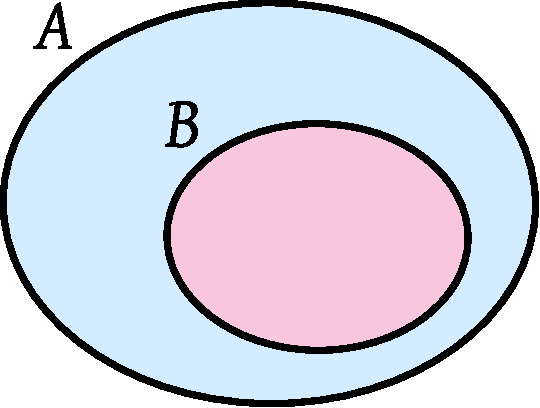
\includegraphics[width=0.8\marginparwidth]{wikipedia_Subset-2.pdf}
\caption{B is a subset of A.  Figure derived from \url{http://upload.wikimedia.org/wikipedia/commons/9/9c/Subset-2.svg}}
\label{fig:subset}
\end{marginfigure}


\bigskip

In probability, an \textbf{event} is the result of an experiment, like picking a random nucleotide.  Events are subsets of the sample space

 For example, if you randomly pick a single nucleotide from a genome, the sample space is \set{A,C,G,T}, and the four possible events are: \set{A}, \set{C}, \set{G}, and \set{T}.

\iffalse
\Question{Suppose you're picking random dinucleotides  from a DNA sequence. Write down 5 possible dinucleotide events.  Be sure to use set notation.}

\Question{Is \set{TT} a possible dinucleotide event here? (explain why/why not)}
\fi


\section{Probability}
\label{sec:probability}

\subsection{Definition of Probability}
\label{sec:defin-prob}
There \marginnote{Believe it or not, until fairly recently there was a very long and very ugly fight between statisticians on the \textit{meaning} of probability.} are several definitions of probability that mean wildly different things.   For us here today, we're focusing on the following definition, which gives the probability of $A$ occurring:


\begin{equation}
\label{eq:defProbability}
P(A) = \frac{\text{Number of ways event A can occur}}{\text{Size of sample space}}
\end{equation}

\bigskip

\samepage{For example, we can analyze the probability of a having a baby girl\marginnote{Assume just one baby.  No twins, no triplets, no quadruplets, \ldots}.  The sample space is \set{girl, boy}, and the event is the set \set{girl}.  That gives:

\[
P(girl) = \frac{1}{2}
\]
}

You can write probability in several ways.  The following are equivalent and all are fine to use:
\[
P(girl) = \frac{1}{2} = 0.5 = 50\%
\]

\bigskip
Notice that from \eqref{eq:defProbability} above, any probability must be between 0~and~1.  If you calculate a probability and it's outside this range, you know that something went wrong.

\Question{What's an example of a situation with a probability of~0?  Show the answer using \eqref{eq:defProbability}.}

\Question{What's an example of a situation with a probability of~1?  Show the answer using \eqref{eq:defProbability}.}


\subsection{Probability Trees}
\label{sec:probability-trees}


We can visualize probability with a tree diagram.  Here's the probability tree for having a baby girl or boy.  The \textcolor{blue}{blue} fractions show probabilities:

\medskip

    \begin{tikzpicture}[grow=right,level distance=2.5cm,
                        every child node/.style={tree node}, 
                        tree node/.style={rectangle, rounded corners, draw},
                        level/.style={sibling distance=35mm/#1}]

        \node[tree node] {Start here}
          child {node {Girl} 
            edge from parent node[anchor=north] {\color{blue}$\frac{1}{2}$}}
          child {node {Boy}
            edge from parent node[anchor=south] {\color{blue}$\frac{1}{2}$}}
         ;
    \end{tikzpicture}

\bigskip\bigskip


Here's a probability tree of picking a random nucleotide :\\*~\\*
    \begin{tikzpicture}[grow=right,
                        level distance=3.cm,
                        every child node/.style={tree node}, 
                        tree node/.style={rectangle, rounded corners, draw},
                        level 1/.style={sibling distance=20mm}]

        \node[tree node] {Start here}
          child {node {A} 
            edge from parent node[anchor=south,very near end] {\color{blue}$\frac{1}{4}$}}
          child {node {C}
            edge from parent node[anchor=south,very near end] {\color{blue}$\frac{1}{4}$}}
          child {node {G}
            edge from parent node[anchor=south,very near end] {\color{blue}$\frac{1}{4}$}}
          child {node {T}
            edge from parent node[anchor=south,very near end] {\color{blue}$\frac{1}{4}$}}
         ;
    \end{tikzpicture}

\bigskip
\Question{Draw a probability tree of picking a random UMB building. (See above for list of buildings)}

\subsection{Probabilities of Mutually Exclusive Events}
\label{sec:adding-probabilities}

If events are mutually exclusive, \marginnote{\textbf{Mutually exclusive} means that only one of the events can occur.  For example, if you flip a coin, the events \set{head} and \set{tail} are mutually exclusive.} you can \textbf{add the probabilities} to find the probability of \textbf{any of the events occurring}.  For example, in the nucleotide probability tree above, you can compute the probability of hitting \set{A} or \set{G} or \set{C} by adding 
$\left( \frac{1}{4} + \frac{1}{4} + \frac{1}{4} \right) = \frac{3}{4}$.  

\Question{What's the probability of randomly picking a UMB building whose name starts with the letter \textit{C}?  (See above for the set of buildings.  Draw the probability tree to visualize the problem.)}


\Question{I'm thinking of a number from 1 to 7.  What's the probability that my number is 3, 4, or 5?  (Show the probability tree and compute the answer.)}.


\subsection{Complementary Probability}
\label{sec:complementary}

If the probability event of some event $A$ is $P(A)$, then the probability of \textit{A not occurring} is $1-P(A)$.  

For example, if the probability of getting hit by lightning is $\frac{1}{1000}$, then the probability of \textit{not} getting by lightening is $1-\frac{1}{1000} = \frac{999}{1000}$.

\Question{If you pick a random nucleotide in a genome, what's the probability that it's \textit{not} G?  (Show calculation.)}

\Question{The subway runs on schedule 92\% of the time.  You have an important job interview downtown and take the T.  What's the probability that you'll have bad luck and be delayed?  (Show tree and calculation.)}

% \clearpage

\section{Conditional Probability}
\label{sec:compound-events}

\Question{Think carefully about this\ldots\  In an abandoned lab in the basement of McCormack, you find an ancient dusty box labeled Amino Acids, containing 20 bottles that are so old you can't read the labels.  If you randomly pick one of the 20 bottles, what's the probability that it's glutamate?

Next, to narrow down the possibilities, you do some pH titration experiments, and determine that this is one of the two acidic amino acids.  \marginnote{Recall there are two acidic amino acids: aspartate and glutamate.}  Given the results of the pH titration experiment, what's the probability that this bottle contains glutamate?}\label{q:condProbGlutamic}

\Question{Here's a very similar question.  Again, think carefully about this.  Suppose I pick a random nucleotide from a genome and I \textit{also tell you that it's a purine}.  
\marginnote{Recall: the purines are A and G.  \\A great mnemonic is \textit{Pure \textbf{AG}ua.}}
Now, using everything you know about the situation, what's the probability that the nucleotide is G?}\label{q:condProbGuanine}


The last two questions show the idea of \textbf{conditional probability}, which means the probability \textit{given some prior event or information}.
In Question~\ref{q:condProbGlutamic} above, we're really asking, ``What's the probability that this bottle contains glutamate \textit{given} that it's acidic?''  

\bigskip

We write conditional probability with a vertical bar $P(A \mid B)$, and say, ``the probability of $A$ \textit{given} $B$.   For Question~\ref{q:condProbGlutamic}  we can write
\[
P(\text{glutamate}  \mid  \text{it's an acid})
\]

\Question{Rewrite Question \ref{q:condProbGuanine} in English using ``\textit{given}'', and also rewrite it as a formula using the vertical bar notation.}


\subsection{Conditional Probability Trees}
\label{sec:cond-prob-trees}


\bigskip
\begin{samepage}
It's good to visualize conditional probability as a tree.  Here's a tree representing the situation in Question~\ref{q:condProbGuanine}.  The \textcolor{blue}{blue} numbers represent the first piece of information; the \textcolor{red}{red} numbers show probability \textit{given} the first information; the \textbf{bold} numbers show the final probability.

\medskip
\probTree
   {pl={\frac{1}{2}},l=Purine,
    pr={\frac{1}{2}},r=Pyrimidine,
    pll={\frac{1}{2}},ll=A,pjll={\frac{1}{4}},
    plr={\frac{1}{2}},lr=G,pjlr={\frac{1}{4}},
    prl={\frac{1}{2}},rl=C,pjrl={\frac{1}{4}},
    prr={\frac{1}{2}},rr=T,pjrr={\frac{1}{4}}
   }
\end{samepage}



\bigskip

\subsection{\textbf{Joint} Probability That Two Events Occur Together}
\label{sec:probability-that-two}

Often we need to know the \textbf{joint} probability of two events $A$ \textbf{and} $B$ both happening.  Figure~\ref{fig:intersection} shows this idea.
\begin{marginfigure}[1.5cm]
\centering
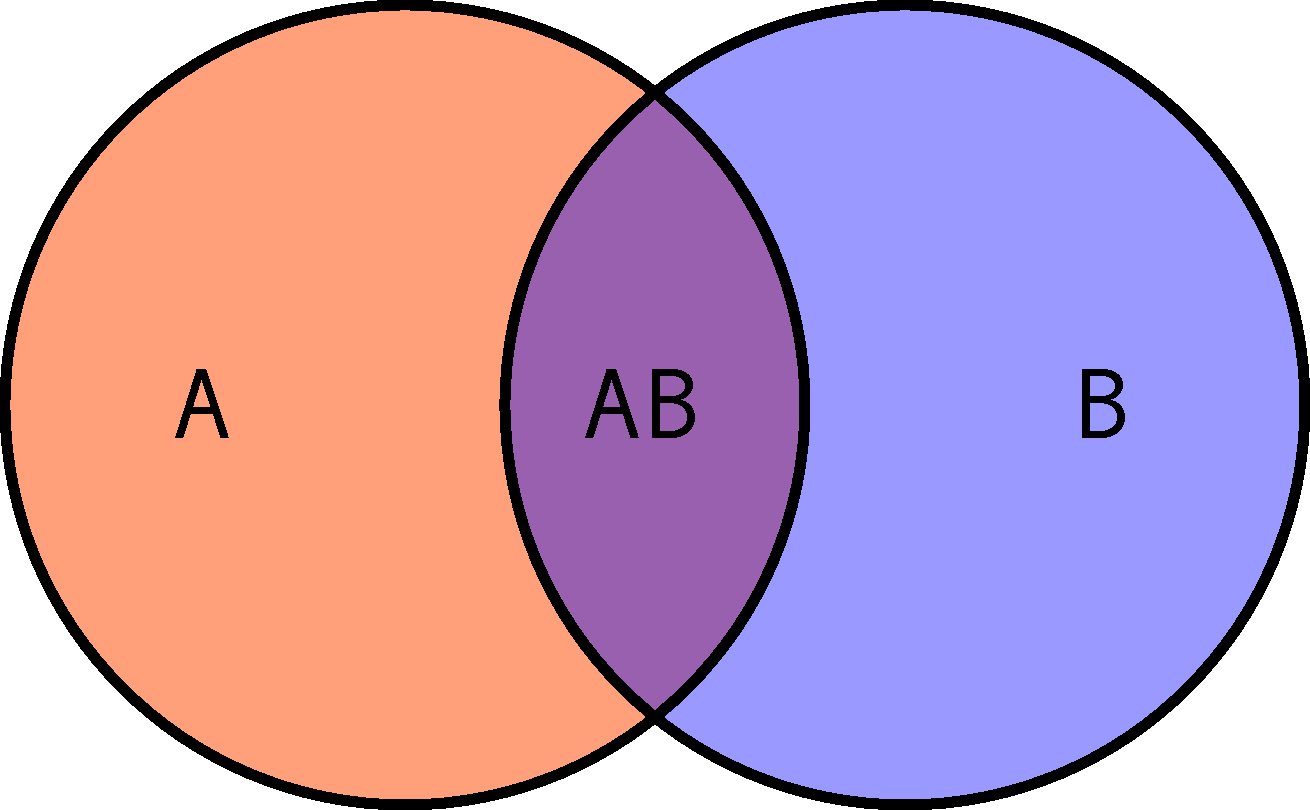
\includegraphics[width=0.7\marginparwidth]{wikipedia_Set_intersection.pdf}
\caption{$AB$ is the joint probability of both $A$ and $B$ occurring.  Figure derived from
\url{http://upload.wikimedia.org/wikipedia/commons/d/da/Set_intersection.svg}}
\label{fig:intersection}
\end{marginfigure}


For example, in genetics, suppose there's a autosomal recessive trait \textbf{f} for obsessive Facebook usage.  Mom's a heterozygote (\textbf{Ff}) and dad's also a heterozygote (\textbf{Ff}), so neither cares about Facebook.  We want to know the probability that little Johnny inherited \textbf{f} from mom \textbf{and} inherited \textbf{f} from dad.   In other words, we want to know the probability that Johnny is homozygous (\textbf{ff}) for the recessive trait.  


To \marginnote{Some books also use set notation $P(A \cap B)$, some books write $P(A \& B)$, and some books write $P(A \text{ and } B)$.  They all mean the same thing as $P(AB)$.} represent the joint probability of two events $A$ \textbf{and} $B$ both, we write $P(AB)$.     To compute the joint probability, use this equation

\begin{equation}
\label{eq:jointProbability}
P(AB) = P(A)  \times  P(B \mid A)
\end{equation}


In the Facebook example, we'll compute the joint probability of \textbf{ff} given the mother's genotype:
\[
P(\textbf{ff}) = P(\text{got \textbf{f} from mom}) \times
                 P(\text{child is \textbf{ff}}  \mid  \text{got \textbf{f} from mom})
\]

\medskip
Here's the probability tree.  The \textcolor{red}{red} probabilities indicate the probability of inheriting a particular allele from dad.

\probTree
   {pl={\frac{1}{2}},l=\textbf{F} from mom,
    pr={\frac{1}{2}},r=\textbf{f} from mom,
    pll={\frac{1}{2}},ll=FF,pjll={\frac{1}{4}},
    plr={\frac{1}{2}},lr=Ff,pjlr={\frac{1}{4}},
    prl={\frac{1}{2}},rl=fF,pjrl={\frac{1}{4}},
    prr={\frac{1}{2}},rr=ff,pjrr={\frac{1}{4}}
   }

\medskip
Notice that the conditional probability tree gave us the classic Mendelian genotypic 1:2:1 Mendelian ratios, and the classic Mendelian phenotypic 1:3 ratios!  Is that cool or what?


\Question{Uncle Ted \marginnote{Hypochondriacs believe they have a disease when they're actually healthy.} is a severe hypochondriac who believes that he has \textbf{both} malaria \textbf{and} HIV.  You have a brilliant idea to cure Ted's hypochondria: Give him a probability tree that shows the minuscule probability that he has both diseases. Sketch out a probability tree for Ted's two imagined diseases, and make up some tiny probabilities along the edges of the tree.  Given those tiny probabilities, compute the final joint probability that Ted has both diseases.  What are the numbers you show Ted?}  

\section{Bayes Theorem}
\label{sec:bayes-theorem}

Suppose you take a blood test and the results come back positive for a serious disease.   Don't panic yet.  It's possible that the result is a \textbf{false positive}.  The are lots of examples of false positives:
\begin{itemize}
\item The weather forecast predicted rain, but there was no rain.
\item The jury convicted an innocent person based on a false fingerprint match.
% \item You want to read about the Boston Red Sox so you Googled for \textit{sox}, and Google returned thousands of pages about footwear.
\item You wrote a computer algorithm to predict protein $\alpha$-helices.  You put in a sequence, the program predicted it was an $\alpha$-helix, but in real biology it's a $\beta$-pleated sheet.

\item You took a mandatory drug test for employment, and even though you've never used illegal drugs, the test came back positive.
\end{itemize}

\Question{Find three other examples of false positives?}

Obviously, after getting a positive test result for a disease,  we really want to know the probability of actually having the disease.  We can represent that as a conditional probability:
\[
P(\text{actually having the disease}  \mid  \text{positive on test})
\]

We can represent that conditional probability as a probability tree.  Figure~\ref{fig:Spiegelhalter2011a} shows a probability tree of breast cancer false positives.  First look at Part A of Figure~\ref{fig:Spiegelhalter2011a}, which shows the results of screening 1000 women for breast cancer.  

\Question{In Part A of Figure~\ref{fig:Spiegelhalter2011a}, 
\marginnote{Hint: Focus just on the disease status, and ignore the test results}
what percentage of women \textit{actually have} breast cancer? (show your calculation)} 

\Question{In Part A of Figure~\ref{fig:Spiegelhalter2011a}, what percentage of women \textit{with} breast cancer test positive?  (Show your work.) On the surface, does that seem like a pretty good diagnostic test?}  

\Question{In Part A of Figure~\ref{fig:Spiegelhalter2011a}, what percentage of women \textit{without} breast cancer test negative?  (Show your work.)  On the surface, does that seem like a pretty good diagnostic test?}  

The big surprise comes in Part B of Figure~\ref{fig:Spiegelhalter2011a}.  We want to know 
\textit{Of the women who test positive, what percentage actually have breast cancer?}  To find that, we compute 
\[
P(\text{breast cancer}  \mid  \text{positive test}) = \frac{\text{number of women with breast cancer \textbf{and} test positive}}
{\text{total number of women who test positive}}
\]

\Question{Compute $P(\text{breast cancer}  \mid  \text{positive test})$.  Now, what do you think about this medical screening test?}

\Question{Look at In Part A of Figure~\ref{fig:Spiegelhalter2011a} again and think carefully about this\ldots\   We know that most women with breast cancer test positive (left half of Part A), and most healthy women test negative (right half of Part A), so the test seems pretty good.  \marginnote{\textbf{\large\color{red}Big hint}: in general, $P(A \mid B) \neq P(B \mid A)$.  \mbox{$P(\text{cancer} \mid \text{test +}) \neq P(\text{test +} \mid \text{cancer})$} } So, why is there such a high false positive rate?}

\subsection{Closing Thought on Bayes Theorem}
\label{sec:clos-thoughts-bayes}

If you've taken a standard probability course, you learned Bayes theorem written algebraically as
\[
P(A \mid B) = \frac{P(B \mid A)\,P(A)}{P(B)}.
\]

A 1998 \marginnote{The problem goes way beyond doctors.  Lawyers and judges are also confused by Bayes theorem, check out the \textit{Prosecutor's Fallacy}.}    study showed that only 10\% of physicians, using this standard algebraic Bayes formula, got the right answers to probability problems like those in Figure~\ref{fig:Spiegelhalter2011a} \citep{Gigerenzer1995a,Hoffrage1998}!  So, if that 1998 study reflects the population of today's physicians, you have a 90\% chance of getting wrong information from your doctor!

In analyzing Figure~\ref{fig:Spiegelhalter2011a}, we took a visual approach to Bayes theorem.  
Later this semester, in a regular lecture, we'll see another simple, non-algebraic approach to computing Bayes theorem using a table instead of a tree.


\begin{figure*}
\centering
\igw{0.9}{Spiegelhalter2011a_fig4.jpg}
\caption{Image source: \citep{Spiegelhalter2011a}}
\label{fig:Spiegelhalter2011a}
\iffalse
Caption from journal:

Fig. 4. Visualizations of the predictive accuracy of a screening test. (A) Tree diagram showing the consequences for 1000 women attending mammography screening from a population with 1\% prevalence of the disease, when the screening test correctly classifies 90\% of women with cancer and 90\% of women without cancer. Although nearly all the women with cancer are detected, they are greatly outnumbered by false-positive tests arising from those without cancer. (B) Icon array of the same information, which shows explicitly that out of 108 positive tests, only 9 (8\%) would be expected to reveal breast cancer.
\fi
\end{figure*}

\bibliographystyle{plain}
\bibliography{unified_bib}

\end{document}


%%%%%%%%%%%%%%%%%%%%%%%%%%%%%%%%%%%%%%%%%%%%%%%%%%%%%%%%%%%%%%%%%%%%%%

% How to do good tables
\iffalse
\begin{tabular}%  requires array
  {l>{\raggedright\hspace{0pt}}p{0.6\textwidth}}
  \toprule
  \textbf{Count} & \textbf{Description}\tnl
  \midrule
  100 & This is a test of the emergency broadcasting system.  If this had been an actual emergency\ldots \tnl
  \bottomrule
\end{tabular}
\fi


%%% Local Variables: 
%%% mode: LaTeX
%%% mode: orgstruct++
%%% TeX-PDF-mode: t
%%% End: 


%%% Local Variables: 
%%% mode: latex
%%% TeX-master: t
%%% End: 
